\chapter{Technische Grundlagen}
\label{cha:Technische-Grundlagen}

In diesem Kapitel werden die technischen Grundlagen beschrieben, auf denen der MiniJava"=Compilers aufgebaut ist. Dazu zählen primär WebAssembly und ANTLR. Weiters wird kurz auf die wichtigsten Hilfstechnologien eingegangen. Außerdem wird anhand ausgewählter Beispiele gezeigt, welche aktuellen Technologien WebAssembly bereits einsetzen oder unterstützen.

\section{WebAssembly}
WebAssembly ist ein Bytecode mit dem Ziel, eine sprachunabhängige Plattform für das Web zu ermöglichen \cite{WebAssemblyWebsite} \cite{WebAssemblySpecification}. So können andere Programmiersprachen (wie zum Beispiel C, C++ oder Rust) und hochperformante Anwendungen in das Web gebracht werden.

\subsection{Hintergrund und Motivation}
Aktuelle Browser unterstützen ausschließlich JavaScript, daher musste bisher der Quelltext anderer Programmiersprachen mit einen Transpiler in JavaScript konvertiert werden. Bei beispielsweise TypeScript übernimmt diese Aufgabe der TypeScript"=Compiler \emph{tsc} \cite{TypeScript}.

JavaScript muss im Browser zur Laufzeit interpretiert werden, gegenbenfalls wird auch ein Just"=In"=Time"=Compiler verwendet \cite{MDNJavaScript}. Dies ist natürlich mit einem gewissen Mehraufwand verbunden. Hier verspricht WebAssembly Performanceverbesserungen, da der Bytecode einfacher geladen (verglichen mit dem Parsen einer Skriptsprache) und effizienter ausgeführt werden kann \cite{WebAssemblySpecification}.

Man könnte auf den ersten Blick vermuten, dass WebAssembly aufgrund des ähnlichen Namen etwas mit \emph{Assembler} gemeinsam hat und man sich daher Gedanken zur Sicherheit machen müsste. Aber deren ist nicht so und WebAssembly gibt ein klares Sicherheitsmodell vor: Vereinfacht beschrieben läuft sämtlicher WebAssembly"=Bytecode im Browser in einer isolierten Umgebung und besitzt nicht mehr Rechte beim Ausführen als JavaScript"=Quelltext \cite{WebAssemblyWebsite} \cite{WebAssemblyW3CPressStandard}.

Im Rahmen eines \emph{Minimum Viable Product} (MVP) entstand die erste Version für WebAssembly, in der nur die notwendigsten Funktionalitäten implementiert wurden, um mit WebAssembly überhaupt arbeiten zu können. \cite{WebAssemblyWebsite}. WebAssembly wird seit 2017 in den vier großen Browsern (Mozilla Firefox, Google Chrome, Apple Safari und Microsoft Edge) unterstützt. Seit Dezember 2019 ist WebAssembly ein offizieller Web"=Standard des W3C (World Wide Web Consortium) \cite{WebAssemblyW3CPressStandard}.

WebAssembly trifft in der Spezifikation keine Annahmen über die Laufzeitumgebung. Auch wenn das derzeit primäre Einsatzgebiet das Web ist, ist es durchaus denkbar, dass WebAssembly auch andersweitig eingesetzt wird. WebAssembly wurde auch so entworfen, dass nicht einmal JavaScript für die Laufzeitumgebung notwendig ist \cite{WebAssemblyWebsite}.

\subsection{Konzepte}
\label{subsec:WebAssembly-Konzepte}
WebAssembly"=Bytecode stellt eine elementare Programmiersprache dar. In der Spezifikation werden für diese einige Konzepte \cite{WebAssemblySpecification} definiert. Nachfolgend werden diese vorgestellt und erklärt.

\begin{description}
    \item[Datentypen] WebAssembly definiert vier Datentypen, zwei für Ganzzahlen und zwei für Fließkommazahlen, jeweils in einer 32"=Bit- und 64"=Bit"=Variante. Der 32"=Bit"=Ganzzahltyp wird auch für Wahrheitswerte und für Speicheradressen verwendet. Die Ganzzahltypen können sowohl für vorzeichenbehafte und vorzeichenlose Zahlen verwendet werden, abhängig von den konkreten Operation darauf werden sie entsprechend interpretiert. Die zwei Ganzzahltypen werden mit \lstinline{i32} und \lstinline{i64} abgekürzt, die zwei Fließkommatypen mit \lstinline{f32} und \lstinline{f64}.
    \item[Instruktionen] Das Laufzeitmodell von WebAssembly basiert auf einer Kellermaschine. Das bedeutet, dass Instruktionen meist Operanden zunächst vom Kellerspeicher herunternehmen, dann die Operation ausführen und am Schluss das Ergebnis wieder auf den Kellerspeicher legen. Standardmäßig werden Instruktionen nacheinander ausgeführt. Es gibt aber auch Instruktionen, die den Kontrollfluss steuern. Einige Instruktionen werden in Abschnitt \ref{subsec:WebAssembly-Instruktionen} detailliert behandelt.
    \item[\emph{Traps}] Instruktionen können (absichtlich oder unbeabsichtigt) Laufzeitfehler in Form von \emph{Traps} erzeugen, die zu einem sofortigen Abbruch der Ausführung führen. Die Behandlung dieser \emph{Traps} erfolgt in der Laufzeitumgebung und nicht direkt in WebAssembly.
    \item[Funktionen] Instruktionen werden in Funktionen gekapselt. Funktionen können beliebig viele Eingangsparameter, maximal ein Funktionsergebnis und beliebig viele lokale Variablen definieren. Funktionen können andere Funktionen oder sich selbst rekursiv aufrufen.
    \item[Tabellen] In Tabellen können derzeit Funktionen abgelegt werden, auf die über einen Index zugegriffen werden kann. Auf diese Art und Weise können beispielsweise Funktionszeiger nachgebildet werden. 
    \item[Linearer Speicher] Linearer Speicher ist ein zusammendhängendes Byte"=Feld, auf das lesend und schreibend zugegriffen werden kann. Der Zugriff erfolgt mit eigenen Instruktionen über einen Index. Beim Erstellen des Speichers wird eine initale Größe definiert, der Speicher kann zur Laufzeit automatisch wachsen.
    \item[Module] In einem Modul werden sämtliche Bestandteile von WebAssembly, darunter Funktionen, Tabellen, Imports und Exports, definiert. Weitere Details zu Modulen finden sich in Abschnitt \ref{subsec:WebAssembly-Module}.
\end{description}

Die Spezifikation fordert nicht, dass Laufzeitumgebungen einen Kellerspeicher zur Auswertung verwalten müssen. Das Programm muss lediglich so ausgeführt werden, als ob es auf einer Kellermaschine laufen würde.

\subsection{Module}
\label{subsec:WebAssembly-Module}
Module sind das Herzstück von WebAssembly. Sämtliche Bestandteile wie beispielsweise Funktionen und deren Implementierung werden als eine Einheit in Form eines Moduls zusammgefasst \cite{WebAssemblySpecification}.

Ein Modul kann textuell oder binär repräsentiert werden. In der Spezifikation werden sämtliche WebAssembly"=Konstrukte in Form einer abstrakten Syntax definiert. Die beiden Darstellungsformen sind somit als Instanzierung dieser abstrakten Syntax zu verstehen. Die abstrakte Syntax definiert eine Baumstruktur. Beide Darstellungeformen sind ineinander umwandelbar. Die binäre Form ist für das \emph{Deployment} vorgesehen, während die textuelle Form als lesbare Darstellung für Menschen gedacht ist \cite{WebAssemblySpecification} \cite{MDNWebAssembly}. Zeilenkommentare sind in der textuellen Darstellung mit \lstinline{;;} möglich.

Die textuelle Darstellung erfolgt in Form von so genannten \emph{S"=Expressions} \cite{WebAssemblySpecification}. Mit diesen können Bäume einfach dargestellt werden. Ein Knoten wird durch \lstinline{(<name> ...)} Ausdrücke beschrieben, zwischen den Klammern befindet sich (durch Leerzeichen getrennt) zuerst der Name/Typ des Knoten, anschließend folgen beliebig viele Werte (zum Beispiel Zahlen oder Zeichenketten) oder Kindknoten \cite{MDNWebAssembly}. In Listing \ref{lst:s-expressions} wird dies anhand eines kleinen Beispiels verdeutlicht.

\lstinputlisting[label={lst:s-expressions}, caption = {Beispiel für \emph{S"=Expressions}: Knoten a hat den Wert 111 und zwei Kindknoten. Diese Kindknoten b und c haben die Werte 222 und 333.}]{src/technischeGrundlagen/sExpressionExample.txt}

Sämtlicher WebAssembly"=Bytecode in dieser Arbeit wird in der textuellen Form mit \emph{S"=Expressions} dargestellt.

In einem Modul können verschiedene Komponenten definiert werden. Nachfolgend wird auf diese im Detail mit Codebeispielen eingegangen.

\begin{description}
    \item[Funktionstypen] Ein Funktionstyp definiert die Schnittstelle einer Funktion. Dabei werden die Datentypen der Eingangsparameter und des Funktionsergebnisses. Auf diese Funktionstypen kann beim Definieren von Funktionen über einen Index zugegriffen werden. Beispielsweise würde der Typ einer Funktion, die zwei 32"=Bit"=Ganzzahlen annimmt und eine 32"=Bit"=Fließkommazahl liefert folgendermaßen definiert werden: \lstinputlisting{src/technischeGrundlagen/modulesType.wat}
    \item[Funktionen] Eine Funktion besteht aus der Signatur und einer Folge von Bytecode"=Instruktionen. Die Signatur kann in der textuellen Darstellung direkt bei der Funktion definiert werden. Alternativ kann ein bestehender Funktionstyp referenziert werden. In einer Funktion können beliebig viele lokale Variablen definiert werden. Angenommen der vorher definierte Funktionstyp wäre über den Index \lstinline{3} erreichbar, könnte man auf folgende zwei Arten eine Funktion mit einer lokalen Variable (64"=Bit Ganzzahl) definieren: \lstinputlisting{src/technischeGrundlagen/modulesFunc.wat}
    Eine Funktion ist über einen Index adressierbar. Dieser Index wird über die Definitionsreihenfolge der Funktionen festgelegt, also erhält die 1. Funktion den Index 0, die 2. Funktion den Index 1 usw.
    \item[Tabellen und Einträge] Diese Funktionsindizes können selbst wieder in Tabellen hinterlegt werden. Damit könnten beispielsweise indirekte Funktionsaufrufe (vergleichbar mit Funktionszeigern) umgesetzt werden. Da für diese Arbeit dieses Konzept nicht relevant ist, wird darauf nicht weiter  eingegangen.
    \item[Linearer Speicher und dessen Initialisierung] Linearer Speicher kann direkt im Modul definiert werden, dabei wird eine Initalgröße (in Anzahl der \emph{Pages}, eine \emph{Page} ist 64KiB groß) angegeben. Der initale Inhalt des Speichers wird über das \lstinline{data}"=Konstrukt definiert. Das folgende Codestück zeigt, wie man beispielsweise einen Speicher definiert (mit Mindestgröße einer Page) und die Zeichenkette \lstinline{"Hello"} an Index 0 ablegt: \lstinputlisting{src/technischeGrundlagen/modulesMemory.wat}
    \item[Globale Variablen] Auf eine globale Variable kann von allen Funktionen aus zugegriffen werden. Eine globale Variabe kann konstant oder veränderbar definiert werden und muss initialisiert werden. Nachfolgend ein Beispiel für zwei 32"=Bit"=Ganzzahlvariablen, einmal konstant und einmal veränderbar. Beide Variablen werden mit \lstinline{123} initialisiert: \lstinputlisting{src/technischeGrundlagen/modulesGlobal.wat}
    \item[Start-Funktion] Jedes Modul kann eine Funktion definieren, die beim Instanzieren des Moduls aufgerufen wird. Die Funktion wird aufgerufen, sobald Tabellen und Speicher initialisiert wurden. Die aufzurufende Funktion wird über den Index angegeben. Nachfolgend sieht man, wie beispielsweise die Funktion mit Index \lstinline{12} als Startfunktion definiert wird: \lstinputlisting{src/technischeGrundlagen/modulesStart.wat}
    \item[Importe] Funktionen, Tabellen, Speicher und globale Variablen können von der Laufzeitumgebung zur Verfügung gestellt werden. Ein Import besteht aus drei Teilen: aus einem Modulnamen, Objektnamen und Objektdefinition. Der Modulname ist nicht mit einem WebAssembly- oder JavaScript"=Modul gleichzusetzen, Modulname und Objektname bilden gemeinsam einen zweistufigen Bezeichner, der flexibel nach Bedarf verwendet werden kann. So würde man beispielsweise die Funktion \lstinline{env.println} importieren, der Funktionstyp wäre hier mit Index \lstinline{1} definiert: \lstinputlisting{src/technischeGrundlagen/modulesImport.wat}
    Über Importe kann in WebAssembly direkt nach außen kommuniziert werden. Auf diese Art können beispielsweise Konsolenausgaben umgesetzt werden.
    \item[Exporte] Funktionen, Tabellen, Speicher und globale Variablen können auch der Laufzeitumgebung zugänglich gemacht werden. Die Definition eines Exports ist etwas einfacher als die eines Imports, da hier kein Modulname notwendig ist. So würde man beispielsweise die Funktion mit Index 3 als \lstinline{main} exportieren: \lstinputlisting{src/technischeGrundlagen/modulesExport.wat}
    Mit Exporte kann die Umgebung mit dem WebAssembly"=Modul kommunizieren. Die Umgebung kann dadurch beispielsweise Funktionen im Modul aufrufen.
\end{description}

\subsection{Instruktionen}
\label{subsec:WebAssembly-Instruktionen}
WebAssembly unterstützt eine Reihe von elementaren Bytecode"=Instruktionen. Instruktionen können zur Compilezeit festgelegte Argumente annehmen. Nachfolgend wird auf einige ausgewählte Instruktionen im Detail eingegangen. Eine vollständige Liste aller Instruktionen findet sich in der WebAssembly"=Spezifikation \cite{WebAssemblySpecification}. (Anmerkung: Die meisten Instruktionen existieren in Ausprägungen für jeden der vier elementaren Datentypen. Die nachfolgenden Beispiele werden nur anhand des 32"=Bit"=Ganzzahltyps gezeigt, \lstinline{i32} könnte man somit mit einem anderen Datentyp ersetzen.)

Die Instruktion \lstinline{i32.const} legt zur Laufzeit eine zur Compilezeit definierte Konstante auf den Kellerspeicher, zum Beispiel: \lstinline{i32.const 123}.

Lokale Variablen lassen sich mit \lstinline{local.get} und \lstinline{local.set} lesen und schreiben. Die lokalen Variablen werden ab \lstinline{0} beginnend nummeriert. Hat eine Funktion Parameter, so zählen die Parameter ebenfalls zu den lokalen Variablen. Der erste Parameter bekommt die Nummer \lstinline{0}, danach folgen die lokalen Variablen.

\lstinline{local.get} liest den Wert der angeforderten lokalen Variable und legt den Wert auf den Kellerspeicher. \lstinline{local.set} holt einen Wert vom Kellerspeicher und speichert diesen in die angegebene Variable. In Listing \ref{lst:wasm-locals} wird das Lesen der ersten lokalen Variable und das Schreiben ihres Werts in die zweite lokale Variable dargestellt, dies entspricht einer einfachen Zuweisung wie \lstinline{a = b}. 

\lstinputlisting[label={lst:wasm-locals}, caption={Lesen und Schreiben lokaler Variablen}]{src/technischeGrundlagen/instructionsLocal.wat}

Für das Rechnen mit Variablen bietet WebAssembly eine Reihe an binären Operationen an. Diese nehmen jeweils die obersten zwei Werte vom Kellerspeicher herunter (Operanden), wenden auf diese die Operation an und legen anschließend das Ergebnis oben auf den Kellerspeicher. Hier drei Beispiele für solche Instruktionen: \lstinline{i32.add} (Addieren), \lstinline{i64.and} (Bitweises Und), \lstinline{f32.le} (Kleiner oder gleich, \emph{lower or equal}).

Weiters gibt es einige strukturierte Instruktionen zur Steuerung des Kontrollflusses. Die einfachste ist die binäre Verzweigung, sie besteht aus drei Instruktionen: \lstinline{if}, \lstinline{else} und \lstinline{end}. Die \lstinline{if}"=Instruktion nimmt einen Wert vom Kellerspeicher. Ist dieser ungleich 0, also \emph{wahr}, werden die Instruktionen zwischen \lstinline{if} und \lstinline{else} ausgeführt. Ist der Wert am Kellerspeicher gleich 0, \emph{falsch}, werden die Instruktionen zwischen \lstinline{else} und \lstinline{end} ausgeführt. In Listing \ref{lst:wasm-if-else-end} ist ein Beispiel dargestellt.

\lstinputlisting[label={lst:wasm-if-else-end},caption = {Beispiel einer binären Verzweigung: Abhängig vom Wert in der ersten lokalen Variable wird \lstinline{1} oder \lstinline{2} in die zweite lokale Variable geschrieben. Rechts daneben ist als Kommentar dazu äquivalenter Pseudocode dargestellt.}]{src/technischeGrundlagen/instructionsIfElseEnd.wat}

Zusätzlich zu der binären Verzweigung sind auch Sprünge möglich. Es ist allerdings nicht möglich, zu jeder beliebigen Instruktion im Bytecode zu springen. Sprungziele werden mit \lstinline{block ... end} oder \lstinline{loop ... end} definiert. Dabei wird beim Betreten des Bereichs ein Sprungziel auf den Kellerspeicher gelegt. Beim Verlassen des Bereichs wird das Sprungziel wieder vom Kellerspeicher genommen. Somit sind die Sprungziele nur innerhalb des Bereichs gültig. Das Sprungziel ist bei \lstinline{block} das Ende des Bereichs, bei \lstinline{loop} der Anfang des Bereichs. Einen (unbedingten) Sprung kann man mit der \lstinline{br}"=Instruktion durchführen. Für einen bedingten Sprung ist die \lstinline{br_if}"=Instruktion vorgesehen, dabei wird ein Wert zunächst vom Kellerspeicher genommen. Nur wenn dieser wahr (ungleich 0) ist, wird gesprungen. Beide Sprunginstruktionen erwarten als Argument eine Zahl \lstinline{n}. Die Instruktion führ dann einen Sprung zum \lstinline{n}"=ten Sprungziel am Kellerspeicher durch. Diese Instruktionen können für Schleifen eingesetzt werden. In Listing \ref{lst:wasm-loop} ist ein Beispiel dargestellt.

\lstinputlisting[label={lst:wasm-loop}, caption = {Beispiel für eine einfache Schleife: Am Anfang der Schleife wird der Wert der ersten lokalen Variable ausgelesen. Ist dieser wahr, wird die Schleife verlassen. Am Ende der Schleife wird unbedingt zum Anfang der Schleife gesprungen. Rechts daneben ist als Kommentar dazu äquivalenter Pseudocode dargestellt.}]{src/technischeGrundlagen/instructionsBranches.wat}

Funktionen können mit der \lstinline{call}"=Instruktion aufgerufen werden. Die Instruktion benötigt als Argument den Index der aufzurufenden Funktion, zum Beispiel: \lstinline{call 1}. Falls die aufgerufene Funktion einen Rückgabewert liefert, liegt dieser nach dem Funktionsaufruf auf dem Kellerspeicher. Daher muss in der Implementierung einer Funktion mit Rückgabewert dieser am Ende der Funktion auf den Kellerspeicher gelegt werden.

Eine Funktion kann frühzeitig mit der \lstinline{return}"=Instruktion verlassen werden. Liefert die Funktion einen Rückgabewert, muss dieser vor der \lstinline{return}"=Instruktion auf den Kellerspeicher gelegt werden.

Ein Laufzeitfehler kann bewusst mit der \lstinline{unreachable}"=Instruktion ausgelöst werden. Diese Instruktion löst immer eine \emph{Trap} aus.

\subsection{Aktueller Entwicklungsstand und zukünftige Entwicklungen}
Wie bereits beschrieben wurde im MVP von WebAssembly nur die allernotwendigste Funktionalität spezifiziert und implementiert. Neue Funktionalitäten durchlaufen einen Standardisierungsprozess \cite{WebAssemblyW3CProcess}. Dieser besteht aus sechs Phasen, die Phasen werden mit 0 beginnend nummeriert:

\begin{enumerate}
    \setcounter{enumi}{-1}
    \item \emph{Pre-Proposal}: Ein Mitglied der \emph{Community Group} hat eine Idee und erstellt eine quasi"=formale Beschreibung. Die \emph{Community Group} stimmt für oder gegen Idee.
    \item \emph{Feature Proposal}: Die Funktionalität wird in einem offiziellen \emph{Repository} aktiv entworfen. Wenn notwendig können Prototypen implementiert werden.
    \item \emph{Proposed Spec Text Available}: Eine vollständige Spezifikation in Englisch ist nun vorhanden. In dieser Phase wird an mindestens einer Implementierung entwickelt, sodass Tests mit dieser ausgeführt werden können. Diese Tests werden in einer Testsuite zusammengefasst.
    \item \emph{Implementation Phase}: Die Testsuite ist nun vollständig und mindestens eine Implementierung durchläuft diese fehlerfrei. Nun müssen sogenannte \emph{Embedder} die Funktionalität implementieren. Die Spezifikation wird weiter verfeinert. Die Referenzimplementierung und Werkzeuge werden um die neue Funktionalität ergänzt.
    \item \emph{Standardize the Feature}: Nun sind einige Implementierungen vollständig und die Spezifikation ist eingefroren, nur noch kleine kosmetische Anpassungen werden vorgenommen. Ab jetzt übernimmt die \emph{Working Group}. Regelmäßig wird über die Nützlichkeit der Funktionalität abgestimmt.
    \item \emph{The Feature is Standardized}: Die Funktionalität ist fertiggestellt und wurde in die Spezifikation aufgenommen.
\end{enumerate}

Sämtliche aktive Entwicklungen werden in einem GitHub"=\emph{Repository} zusammengefasst \cite{WebAssemblyProposals}.
Einige davon haben bereits die Implementierungsphase (4) erreicht, beispielsweise Unterstützung für Referenzdatentypen. \emph{Threads} befinden sich beispielsweise erst in Phase 2. Interessante Funktionalitäten wie \emph{Garbage Collection} oder \emph{Interface Types} (diese sollen dabei helfen, die Interoperabilität mit Web"=APIs zu verbessern \cite{WebAssemblyInterfaceTypes}) sind erst in Phase 1.

\subsection{\emph{WebAssembly Binary Toolkit}}
Das \emph{WebAssembly Binary Toolkit} (WABT) ist eine Sammlung an Werkzeugen, die EntwicklerInnen im Kontext von WebAssembly unterstützen sollen \cite{WABT}. Dazu zählen Werkzeuge zum Analysieren, Validieren und Dekompilieren von WebAssembly"=Modulen. Zwei im Rahmen dieser Arbeit nützliche Werkzeuge sind \lstinline{wat2wasm} und \lstinline{wasm2wat}, mit denen zwischen der textuellen und binären Repräsentation eines Moduls hin und her konvertiert werden kann. Konkret wird \lstinline{wat2wasm} im MiniJava"=Compiler eingesetzt, um das binäre WebAssembly"=Modul zu generieren.

\subsection{JavaScript-API}
\label{subsec:WebAssembly-JavaScript-API}
JavaScript stellt eine Schnittstelle zur Verfügung, mit der WebAssembly"=Module geladen, kompiliert und ausgeführt werden können \cite{MDNWebAssembly}. In diesem Abschnitt soll ein Überblick über diese Schnittstelle gegeben werden.

Zunächst muss das Modul geladen werden. Dies kann im Browser beispielsweise mit \lstinline{fetch} und in Node.js mit \lstinline{fs.readFile} erfolgen. Mit \lstinline{WebAssembly.compile} wird aus diesen Rohdaten das Modul kompiliert. Im Browser können diese zwei Schritte auch gemeinsam mit \lstinline{WebAssembly.compileStreaming} zusammengefasst werden, dabei wird während des Herunterladens das Modul gleichzeitig kompiliert. Dadurch können schnellere Ladezeiten erreicht werden. Diese Funktion ist allerdings nicht in allen Browsern verfügbar.

Nun wird mit \lstinline{WebAssembly.instantiate} eine Instanz des Moduls erzeugt. Diese Funktion benötigt als weiteren Parameter ein JavaScript"=Objekt, das die Imports definiert. In diesem Import"=Objekt spiegelt sich der zweistufige Bezeichner wieder. So könnte man beispielsweise die in Abschnitt \ref{subsec:WebAssembly-Module} importierte Funktion \lstinline{env.println} bereitstellen:

\lstinputlisting{src/technischeGrundlagen/importObject.js}

Die Schritte Herunterladen, Kompilieren und Instanzieren lassen sich ebenfalls mit der (nicht in allen Browsern unterstützten) Funktion \lstinline{WebAssembly.instantiateStreaming} zusammenfassen.

Man erhält am Ende die Modulinstanz als JavaScript"=Objekt. Dieses Objekt hat die Datenkomponente \lstinline{exports}. Über diese können exportiere Funktionen aufgerufen werden.

In Listing \ref{lst:wasm-js-api} findet sich ein zusammenhängendes Beispiel, um das Zusammenspiel zwischen WebAssembly und JavaScript zu veranschaulichen.

\lstinputlisting[label={lst:wasm-js-api}, caption = {Beispiel aus der MDN"=Dokumentation \cite{MDNWebAssembly}: In JavaScript wird die exportierte Funktion \lstinline{exported_func} aufgerufen, diese ruft wiederum \lstinline{imported_func} auf. Das Programm gibt zur Laufzeit \lstinline{42} auf der Konsole aus.}]{src/technischeGrundlagen/simpleJSAPI.txt}

\section{ANTLR}

ANTLR (ANother Tool for Language Recognition) ist ein von Terence Parr entwickelter Scanner- und Parsergenerator, der Quelltext für diverse Programmiersprachen (darunter Java und C\#{}) generiert \cite{ANTLR4Reference} \cite{ANTLRWebsite}. ANTLR selbst ist in Java geschrieben. Die Programmiersprache, für die Scanner und Parser generiert werden, wird nachfolgend auch als Zielsprache bezeichnet. Unter \emph{ANTLR} ist in der gesamten Arbeit die aktuelle Hauptversion 4 zu verstehen, außer es wird explizit anders angegeben.

\subsection{Parser}

ANTLR ist in der Lage, für jede kontextfreie Grammatik ohne indirekte oder versteckte Linksrekursion einen Parser zu erzeugen \cite{ANTLRALLStar}. Eine indirekte Linksrekursion ist beispielsweise in folgenden Regeln enthalten: $A \rightarrow B.\ B \rightarrow A.$ \cite{ANTLRALLStar}. Eine versteckte Linksrekursion findet sich beispielsweise in diesen Regeln: $A \rightarrow B A.\ B \rightarrow \epsilon.$ \cite{ANTLRALLStar}. Der Parser arbeitet nach dem Prinzip des rekursiven Abstiegs. Das dabei eingesetzt Verfahren heißt ALL(*) (Adaptive LL(*)). In diesem Abschnitt wird das Verfahren nur überblicksmäßig erläutert, weitere Details dazu sind in \cite{ANTLR4Reference}, \cite{ANTLRLLStar} und \cite{ANTLRALLStar} nachzulesen.

ALL(*) basiert auf dem in ANTLR 3 eingesetzten LL(*). LL(*) unterscheidet sich von LL(k) dahingehend, dass die Anzahl der Vorgriffssymbole nicht fixiert ist \cite{ANTLRLLStar}. Beim Treffen einer Entscheidung bei Alternativen wird stattdessen ein regulärer Ausdruck verwendet. ANTLR 3 erzeugt beim Generieren des Parsers für jedes Nonterminalsymbol einen deterministischen endlichen Automat. Gelingt es nicht, einen solchen Automanten zu erzeugen, wird auf \emph{Backtracking} zurückgegriffen.

ALL(*) erweitert die Idee von LL(*): Hier wird der determinische endliche Automat beim Parsen dynamisch erzeugt \cite{ANTLRALLStar}. Beim Erzeugen des Automaten werden die Symbole der tatsächlichen Eingabe verwendet. Beim Treffen zukünftiger Entscheidungen wird der bestehende Automat verwendet oder wenn notwendig erweitert. Der Vorteil gegenüber LL(*) ist, dass beim Aufbau des deterministischen endlichen Automaten zur Laufzeit nur eine endliche Menge an Eingaben berücksichtigt werden muss, während bei LL(*) \emph{alle} Möglichkeiten von potenziellen Eingaben berücksichtigt werden müssen.

ALL(*) kann mit kontextfreien Grammatik ohne indirekte oder versteckte Linksrekursion umgehen \cite{ANTLR4Reference} \cite{ANTLRALLStar}. ANTLR ist jedoch in der Lage, direkte Linksrekursionen aufzulösen. Dadurch lassen sich mathematische Ausdrücke übersichtlicher und kompakter schreiben. Der Vorrang der Operatoren wird durch die Reihenfolge der Alternativen beschrieben: Die Priorität nimmt von oben nach unten ab. Bei den Operatoren wird standardmäßig Linksassoziativität angenommen, benötigt man Rechtsassoziativität, muss dies explizit angegeben werden. So kann aus einer eigentlich mehrdeutigen Grammatik ein eindeutiger Syntaxbaum aufgebaut werden. In Listing \ref{lst:antlr-left-recursion} findet sich ein Beispiel um das zu verdeutlichen.

\pagebreak
\lstinputlisting[label={lst:antlr-left-recursion}, caption = {Beispiel für mathematische Ausdrücke in ANTLR \cite{ANTLR4Reference}}]{src/technischeGrundlagen/antlrMathExpressions.g4}

Insgesamt lassen sich durch das automatische Auflösen von Linksrekursionen und durch ALL(*)"=Grammatiken schreiben, die nicht zu stark auf das darunterliegende Parser"=Verfahren angepasst werden müssen \cite{ANTLR4Reference}. Ein extremes Gegenbeispiel dazu ist die (händische) Transformation einer Grammatik, sodass die daraus entstehende Grammatik LL(1)"=konform ist.

\subsection{Grammatikbeschreibung}

Die Grammatik einer Sprache wird in einer Textdatei mit dem Dateityp \lstinline{g4} beschrieben. In Listing \ref{lst:antlr-listOfNumbers-grammar} ist ein einfaches Beispiel für eine Grammatik, die benannte Zahlenlisten beschreibt, zum Beispiel \lstinline{even[ 2 4 ]}, \lstinline{empty[ ]} oder \lstinline{prime[ 2 3 5 7 ]}. In Abbildung \ref{fig:syntaxtree} wird der Syntaxbaum des Satzes \lstinline{even[ 2 4 ]} dargestellt.

\lstinputlisting[label = {lst:antlr-listOfNumbers-grammar}, caption = {\emph{MyLanguage.g4}}]{src/technischeGrundlagen/MyLanguage.g4}

\begin{figure}[b]
    \centering
    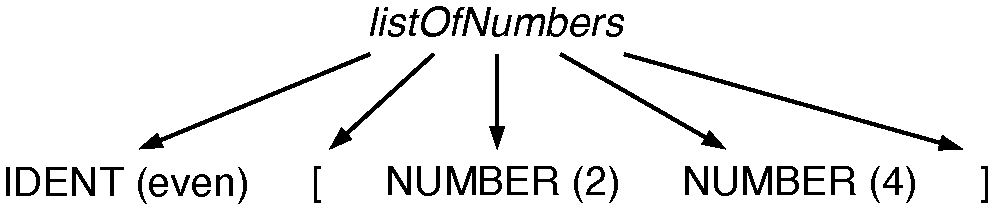
\includegraphics[width=0.6\textwidth]{technischeGrundlagen/syntaxtree}
    \caption{Syntaxbaum des Satzes \lstinline{even[ 2 4 ]}}
    \label{fig:syntaxtree}
\end{figure}

Am Beginn steht der Name der Grammatik. Anschließend folgen Regeln für Nonterminalsymbole und zum Schluss Terminalsymbole. Formatierungen wie Leerzeichen, Zeilenumbrüche usw. können ignoriert werden. Dafür ist das Terminalsymbol \lstinline{WS} (steht für \emph{white space}) zuständig. Mit \lstinline{-> skip} werden in diesem Fall Leerzeichen, Tabulatorzeichen und Zelenendezeichen ignoriert, sodass man sich in der Grammatik darum nicht mehr kümmern muss. Das \lstinline{*}"=Symbol kennzeichnet $0$ bis $n$ Wiederholungen des vorherigen Ausdrucks, das \lstinline{+}"=Symbol kennzeichnet $1$ bis $n$ Wiederholungen.

Beim Parsen entsteht aus einem Eingabetext ein Syntaxbaum. Nonterminalsymbole stellen Knoten in diesem Baum dar, Terminalsymbole sind darin Blattknoten. Kindknoten lassen sich in diesem Syntaxbaum auch benennen. Zu einem \lstinline{listOfNumbers}"=Knoten aus dem obigen Beispiel wird das Terminalsymbol \lstinline{IDENT} mit \lstinline{name} benannt. Der Knoten im Syntaxbaum erhält dann eine Datenkomponente \lstinline{name}, die auf das Terminalsymbol verweist. Es können auch mehrere Kindknoten in einer Liste gespeichert werden (dies erfolgt mit dem Operator \lstinline{+=}), in diesem Fall werden alle \lstinline{NUMBER}-Terminalsymbole in der Datenkomponente \lstinline{numbers} zusammengefasst.

Aus der Grammatikdatei werden Scanner, Parser und weitere Hilfsklassen mit dem ANTLR"=Werkzeug\footnote{\url{https://www.antlr.org/download/antlr-4.8-complete.jar}} erzeugt. Dieser Prozess lässt sich außerdem in Gradle über ein Plugin integrieren \cite{GradleANTLRPlugin}.

\subsection{Integration in Kotlin}

Aus der im vorherigen Abschnitt beschriebenen Grammatik kann mit ANTLR nun Quelltext für die Zielsprache Java erzeugt werden. Die Namen der generierten Dateien beginnen mit dem Grammatiknamen. Der erzeugte Scanner und Parser wird nun in ein eigenes Programm integriert.

Da sich Java von Kotlin aus verwenden lässt, findet sich in Listing \ref{lst:antlr-kotlin-usage} ein Beispiel, wie der generierte Scanner und Parser in Kotlin aufgerufen wird. 

\lstinputlisting[label = {lst:antlr-kotlin-usage}, caption = {Verwendung der generierten ANTLR"=Klassen in Kotlin}]{src/technischeGrundlagen/antlrKotlin.kt}

Zu den einzelnen Zeilen ein paar Details:
\begin{itemize}
    \item In Zeile 1 wird aus dem Inhalt der Datei mit dem Namen \lstinline{"..."} ein Strom an Zeichen erzeugt.
    \item In Zeile 2 wird aus der generierten Klasse \lstinline{MyLanguageLexer} und dem Zeichenstrom ein \lstinline{Lexer}"=Objekt erzeugt.
    \item In Zeile 3 wird aus dem \lstinline{Lexer}"=Objekt ein Strom an Terminalsymbolen (\lstinline{Tokens}) erzeugt.
    \item In Zeile 4 wird aus der generierten Klasse \lstinline{MyLanguageParser} und dem Strom an Terminalsymbolen ein \lstinline{Parser}"=Objekt erzeugt.
    \item In Zeile 5 wird ein Syntaxbaum beginnend mit dem Satzsymbol \lstinline{listOfNumbers} aufgebaut.
\end{itemize}

\pagebreak
\subsection{Semantische Aktionen}

Oft reicht es nicht, lediglich zu überprüfen, ob ein Text in der Sprache der Grammatik enthalten ist. Besonders beim Parsen von Programmiersprachen müssen anhand des konkreten Quelltextes Entscheidungen oder semantische Aktionen getroffen werden. ANTLR bietet hier zwei Ansätze an:

\begin{itemize}
    \item Die Struktur der Sprache wird in einer Grammatik beschrieben. Semantische Aktionen stehen davon getrennt in eigenen Komponenten (\lstinline{Listener} oder \lstinline{Visitor}), die den Syntaxbaum auswerten. Die Grammatik enthält keinen zielsprachenspezifischen Quelltext.
    \item Die Grammatik enthält zielsprachenspezifischen Quelltext in Form von Codeeinschlüssen. Diese Einschlüsse werden im generierten Scanner bzw. Parser eingebettet und später während dem Scannen und Parsen ausgeführt. 
\end{itemize}

Parr empfiehlt, soweit als möglich auf Codeeinschlüsse zu verzichten. Dafür sprechen folgende Argumente \cite{ANTLR4Reference}:
\begin{itemize}
    \item Saubere Trennung von Grammatik und Auswertung im Sinne des \emph{Single-res\-pon\-si\-bi\-li\-ty principle} \cite{AgileSoftwareDevelopmentPPP}.
    \item Da die Grammatik zielsprachunabhängig bleibt, können Scanner und Parser einfacher für andere Zielsprachen aus bestehenden Grammatiken erzeugt werden.
    \item Die Grammatik bleibt übersichtlicher, da Quelltext der Zielsprache nicht mit Grammatikregeln verwoben ist.
\end{itemize}

Dennoch kann es Gründe geben, die für Codeeinschlüsse sprechen:
\begin{itemize}
    \item Wenn nur wenige semantische Aktionen benötigt werden und der Quelltext der gesamten Anwendung so übersichtlicher bleibt.
    \item Um sich das Aufbauen des Syntaxbaums im Arbeitsspeicher zu ersparen. Dies ist zum Beispiel bei performancekritischen Anwendungen wichtig.
    \item Manchmal ist es notwendig, Entscheidungen im Parsevorgang selbst treffen zu müssen (zum Beispiel für \emph{Predicated parsing}).
    \item Die Generierung für mehrere Zielsprachen ist nicht notwendig.
    \item Die Wiederverwendbarkeit der Grammatik steht nicht im Vordergrund.
\end{itemize}

\begin{figure}[b]
    \centering
    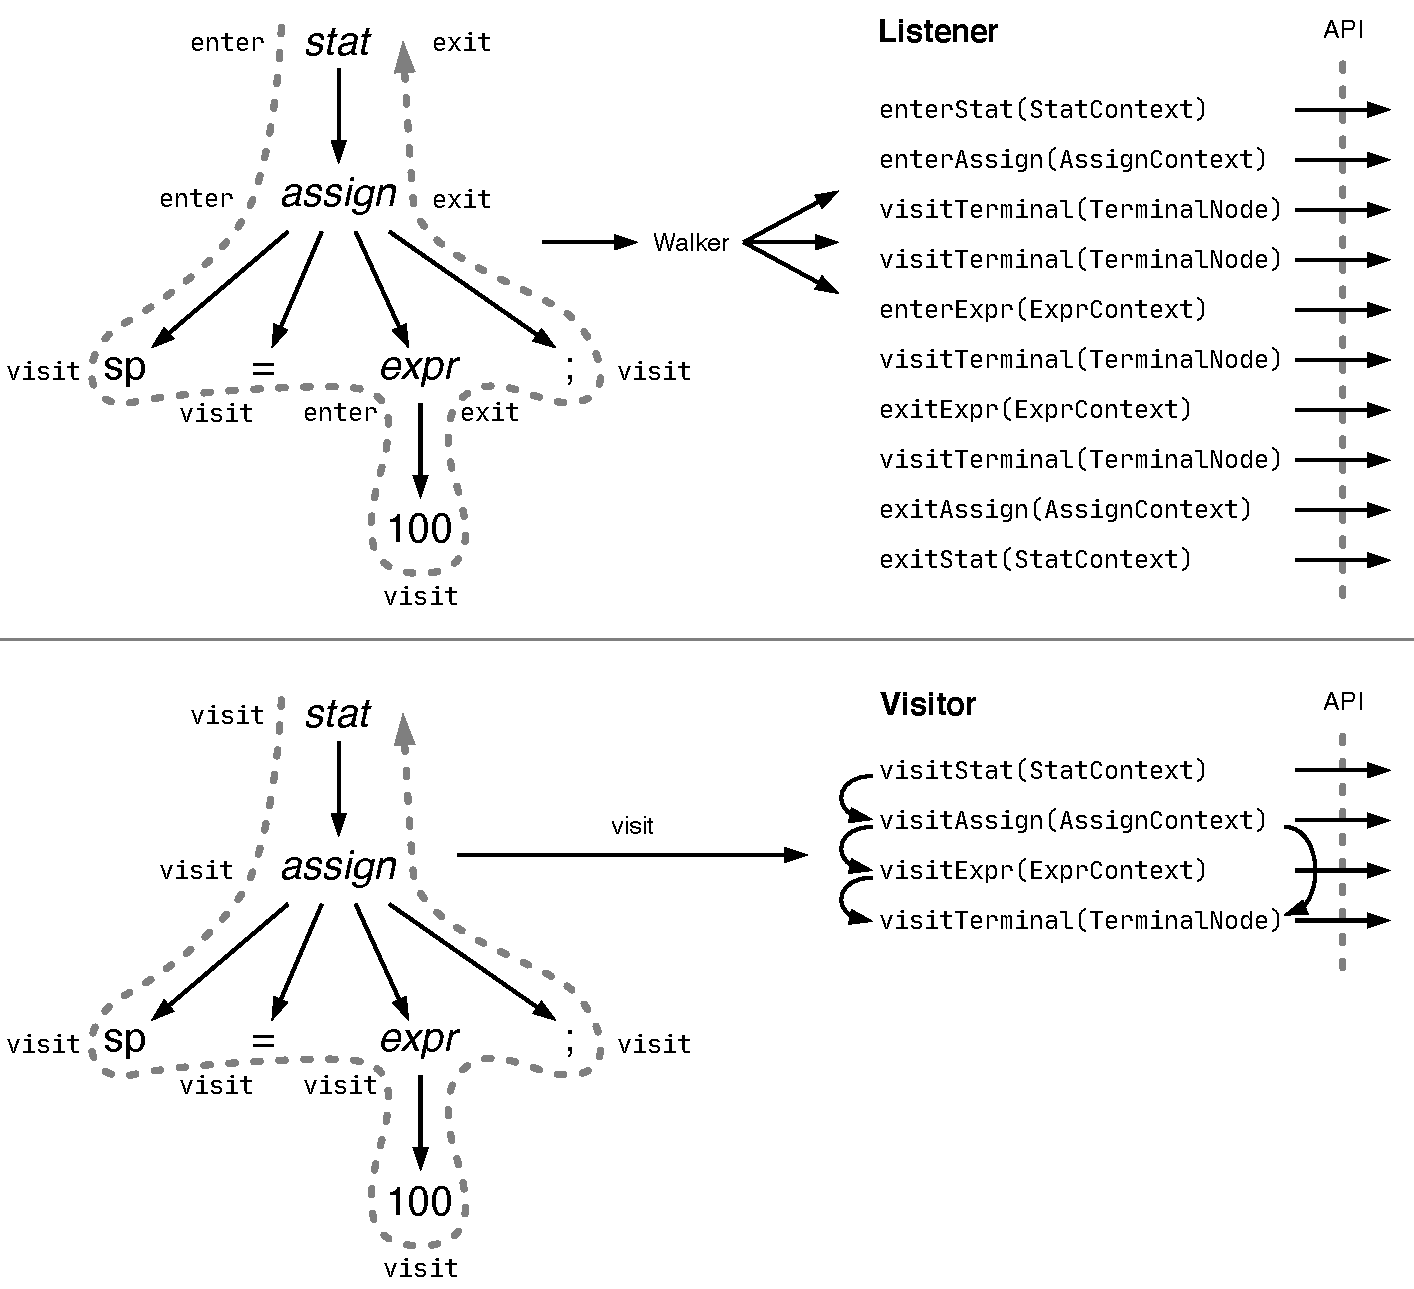
\includegraphics[width=\textwidth]{technischeGrundlagen/listenerVisitor}
    \caption{Abarbeiten des Syntaxbaums des Satzes \lstinline{x = 100;} mit einem \lstinline{Listener} und \lstinline{Visitor} \cite{ANTLR4Reference}}
    \label{fig:listenerVisitor}
\end{figure}

In dieser Arbeit wurde der Ansatz mit sauberer Trennung von Grammatik und Auswertung umgesetzt. Wie bereits erwähnt, bietet ANTLR dafür mit \lstinline{Listener} und \lstinline{Vistor} zwei Möglichkeiten, um den Syntaxbaum auszuwerten. In Abbildung \ref{fig:listenerVisitor} werden die beiden Ansätze visuell gegenübergestellt. Nachfolgend werden die zwei Ansätze im Detail beschrieben.

Die einfachste Art, einen Syntaxbaum abzuarbeiten besteht aus einer Kombination aus einem \lstinline{ParseTreeWalker} und einem \lstinline{Listener}. Das Prinzip ist hier vergleichbar mit dem Verarbeiten von XML"=Dokumenten auf Basis von SAX. ANTLR stellt den \lstinline{ParseTreeWalker} zur Verfügung, der \lstinline{Listener} ist auf Basis eines generierten \emph{Interfaces} selbst zu implementieren. Der Syntaxbaum wird vom \lstinline{ParseTreeWalker} in einer \emph{depth"=first}"=Reihenfolge abgearbeitet. Beim Betreten und Verlassen eines Knoten werden bei Nonterminalsymbolen entsprechende \lstinline{enter}- und \lstinline{exit}"=Methoden des \lstinline{Listeners} aufgerufen, bei Terminalsymbolen gibt es nur die Methode \lstinline{visitTerminal}.

Manchmal ist jedoch etwas mehr Kontrolle notwendig: Zum Beispiel wenn man den Baum in einer anderen Reihenfolge auswerten möchte. Es kann auch sein, dass Teile des Syntaxbaums gar nicht ausgewertet werden müssen. Hier muss basierend auf einem generierten \emph{Interface} ein \lstinline{Visitor} implementiert werden. Für jeden Knotentyp gibt es eine Methode nach dem Schema \lstinline{visitXYZ}. In der Implementierung der \lstinline{visit}"=Methoden muss, sofern erwünscht, aktiv das Abarbeiten von Kindknoten angestoßen werden.

ANTLR generiert zu jedem \lstinline{Listener}- und \lstinline{Visitor}"=\emph{Interface} eine Basisimplementierung, in der beim \lstinline{Listener} alle Methoden leer sind und beim \lstinline{Visitor} alle Kinder abgearbeitet werden. So müssen in eigenen Implementierung nur die relevanten Methoden überschrieben werden.

\pagebreak
\section{Weitere Technologien}

Neben WebAssembly und ANTLR als Kerntechnologien werden für die Implementierung einige Hilfstechnologien benötigt. Auf diese wird in diesem Abschnitt eingegangen.
\subsection{Kotlin}
Kotlin ist eine von JetBrains entwickelte Programmiersprache \cite{KotlinReference}. Kotlin zeichnet sich besonders durch die kompakte Syntax und starke Integration in das bestehende Java"=Umfeld aus. Zusätzlich bietet Kotlin Absicherungen gegen \lstinline{NullPointerExceptions} zur Übersetzungszeit. Wie bei Java wird aus Kotlin beim Kompilieren Bytecode für die \emph{Java Virtual Machine} (JVM) erzeugt. Durch diese enge Interoperabilität kann beim Programmieren mit Kotlin auf die bereits große Menge an Java"=Bibliotheken zurückgegriffen werden.

Die kompakte Syntax von Kotlin gegenüber Java wird anhand eines kleinen Beispiels mit \emph{Data Classes} gezeigt. Mit \emph{Data Classes} können Klassen, die primär nur Daten kapseln, sehr einfach definiert werden, da oft benötigte Methoden wie \emph{Getter}, \emph{Setter}, \lstinline{hashCode}, \lstinline{equals} und \lstinline{toString} automatisch vom Kotlin"=Compiler erzeugt werden. Außerdem wird ein Konstruktor generiert, mit dem alle Datenkomponenten initialisiert werden können. In Java müsste man all diese Methoden händisch schreiben oder von der IDE generieren lassen. In Listings \ref{lst:point-kotlin} und \ref{lst:point-java} wird der Quelltext für die Klasse \lstinline{Point} gezeigt. Die Unterschiede sind deutlich sichtbar.

\lstinputlisting[label = {lst:point-kotlin}, caption = {Die Klasse \lstinline{Point} in Kotlin}]{src/technischeGrundlagen/Point.kt}

\lstinputlisting[label = {lst:point-java}, caption = {Die Klasse \lstinline{Point} in Java. Konstruktor, \emph{Getter}, \emph{Setter}, \lstinline{hashCode}, \lstinline{equals} und \lstinline{toString} wurden von IntelliJ generiert.}]{src/technischeGrundlagen/Point.java}

Kotlin bietet wie bereits erwähnt Absicherungen gegen \lstinline{NullPointerExceptions} zur Übersetzungszeit. Ein einfaches Beispiel dafür findet sich in Listing \ref{lst:npe-kotlin}.

\lstinputlisting[label = {lst:npe-kotlin}, caption = {Beispiel für die Absicherungen gegen \lstinline{NullPointerExceptions}. Die Methode \lstinline{findPoint} liefert als Rückgabewert die Referenz auf ein \lstinline{Point}"=Objekt oder \lstinline{null}, dies wird durch das Fragezeichen gekennzeichnet. Da die lokale Variable \lstinline{point} in Zeile 5 nach dem Aufruf \lstinline{null} sein kann und ein Zugriff auf die \lstinline{x}"=Datenkomponente zu einer \lstinline{NullPointerException} führen könnte, wird ein Übersetzungsfehler ausgelöst. Nach der Prüfung in Zeile 6 kann garantiert werden, dass \lstinline{point} nicht \lstinline{null} ist, somit kann in Zeile 7 gefahrlos auf die Datenkomponente zugegriffen werden.}]{src/technischeGrundlagen/nullSaftety.kt}

Bei MiniJava wird Kotlin als Implementierungssprache des MiniJava"=Compilers eingesetzt. Der von ANTLR generierte Parser (Java"=Quelltext) lässt sich von Kotlin ausgehend problemlos verwenden. Kotlin wurde aufgrund persönlicher Präferenz gewählt, da die tatsächliche Implementierungssprache des Compilers im JVM"=Umfeld keine essenzielle Rolle spielt.

\pagebreak
\subsection{Node.js}
Node.js ist eine JavaScript"=Laufzeitumgebung, die auf der V8"=JavaScript"=Engine aufbaut \cite{NodeJSDocumentation}. Node.js wird unter anderem bei skalierbaren Serveranwendungen eingesetzt, die möglichst viele Verbindungen gleichzeitig abarbeiten können sollen. Node.js unterstützt die JavaScript"=API für WebAssembly (siehe Abschnitt \ref{subsec:WebAssembly-JavaScript-API}).

Bei MiniJava wird Node.js als Laufzeitumgebung für Konsolenanwendungen eingesetzt.

\subsection{JavaScript}
JavaScript ist eine Skriptsprache, die zur Laufzeit interpretiert wird \cite{MDNJavaScript}. Bekannt ist sie vor allem als clientseitige Programmiersprache im Browser für Webseiten. JavaScript ist prototypbasiert und dynamisch typisiert. Weiters besitzt JavaScript nur eine Handvoll an Datentypen, darunter \lstinline{number} für Ganz- und Fließkommazahlen, \lstinline{string} für Zeichenketten, \lstinline{boolean} für Wahrheitswerte, \lstinline{function} für Funktionen und \lstinline{object} für jede Art von Objekten inklusive Feldern. Der Sprachumfang von JavaScript basiert auf der ECMAScript"=Spezifikation.

JavaScript dient bei MiniJava als Bindeglied zu WebAssembly.

\subsection{Gradle}
Gradle ist ein Build"=System, das sich im Java"=Umfeld etabliert hat \cite{Gradle}. Der Build"=Prozess wird dabei deklarativ in der Programmiersprache Groovy beschrieben.

Das Kernelement sind so genannte \emph{Tasks}, die eine definierte Aufgabe erfüllen, beispielsweise Java"=Quelltext kompilieren, Tests ausführen oder ein Java"=Archiv (JAR) erstellen. Zwischen \emph{Tasks} lassen sich Abhängigkeiten definieren, dadurch werden \emph{Tasks} in der richtigen Reihenfolge abgearbeitet, beispielsweise müssen Tests nach dem Kompilieren ausgeführt werden. Weiters können für \emph{Tasks} Eingaben und Ausgaben (das sind Verzeichnisse oder Dateien) definiert werden. Mit diesen Informationen kann Gradle den Build"=Prozess dahingehend optimieren, dass nur diejenigen \emph{Tasks} ausgeführt werden, bei denen es auch sinnvoll ist: Beispielsweise würde es nichts bringen, Java"=Quelltext nocheinmal zu kompilieren, wenn er seit dem letzten Kompilieren nicht verändert wurde.

Gradle baut auf der Abhängigkeitsverwaltung von Maven auf. So lassen sich bestehende Bibliotheken, die zum Beispiel im \emph{Central Repository}\footnote{\url{https://search.maven.org}} verfügbar sind, einfach einbinden.

Bei MiniJava wird Gradle bei der gesamten Implementierung dieser Masterarbeit eingesetzt, sowohl beim Kompilieren des MiniJava"=Compilers selbst, als auch beim Kompilieren MiniJava"=Quelltexte mit dem MiniJava"=Compiler.

\subsection{\emph{webpack}}
\emph{webpack} ist ein Werkzeug, mit dem mehrere JavaScript"=Module, die auf mehrere Dateien aufgeteilt sind, in eine einzige JavaScript"=Datei zusammengebündelt werden können \cite{Webpack}. webpack unterstützt eine Reihe von Modulsystemen, darunter \emph{CommonJS} mit der Anweisung \lstinline{require} oder die \lstinline{import}"=Anweisungen im ES2015"=Umfeld. Weiters kann webpack auch so konfiguriert werden, dass andere Programmiersprachen (wie zum Beispiel TypeScript) ebenfalls in diesen Prozess eingebunden werden können. Diese werden dabei mit einem Transpiler in JavaScript"=Quelltext konvertiert.

Bei MiniJava wird webpack eingesetzt, um beim Einsatz im Browser alle generierten JavaScript"=Dateien in einer gemeinsamen JavaScript"=Datei zusammenzufassen.

\subsection{\emph{JUnit} und \emph{AssertJ}}
\emph{JUnit} ist ein Unit"=Test"=Framework für Java \cite{JUnit}. Testfälle können sehr einfach definiert werden. Es genügt dabei, eine Methode mit der \lstinline{@Test}"=Annotation zu markieren, dann kann sie von JUnit gefunden werden. Weiters lässt sich JUnit direkt in Gradle als Teil des Build"=Prozesses integrieren \cite{Gradle}.

\emph{AssertJ} ist eine Bibliothek zum Schreiben von Assertionen. JUnit bietet diese Funktionalität bereits, jedoch ist der wesentliche Vorteil gegenüber JUnit, dass die Assertionen fast wie ein englischer Satz aussehen. Nachfolgend ein Beispiel dazu:

\lstinputlisting{src/technischeGrundlagen/assertions.java}

Auch wenn der Quelltext etwas länger ist, ist er aussagekräftiger. Außerdem würde man sofort erkennen, wenn man den erwarteten und den tatsächlichen Wert vertauschen würde.

JUnit wird gemeinsam mit AssertJ bei MiniJava zum Testen des Compilers eingesetzt.

\pagebreak
\section{Aktuelle Unterstützung für WebAssembly}
Es gibt bereits eine Reihe von Technologien, die auf WebAssembly aufbauen. In diesem Abschnitt werden drei ausgewählte aktuelle Technologien betrachtet. Es wird dabei der Fokus auf den Einsatz der Technologien und die Art der Integration mit WebAssembly sowie JavaScript gelegt.

\subsection{Emscripten}

Emscripten ist ein Compiler, mit dem sich C/C++"=Quelltext nach WebAssembly übersetzen lässt \cite{Emscripten}. Die grundsätzliche Idee ist, dass sich mit möglichst wenig Aufwand bestehender C/C++"=Quelltext ins Web bringen lässt. Zum Beispiel werden \lstinline{printf}"=Aufrufe automatisch auf die Browser"=Konsole abgebildet. Weitere typische Bibliotheken werden direkt unterstützt, darunter zum Beispiel \emph{Simple DirectMedia Layer} (SDL), OpenGL (über WebGL) und OpenAL (über Web Audio API). Emscripten bietet zusätzlich eine Reihe von eigenen Schnittstellen an, darunter zum Beispiel Anbindungen an HTML 5 und WebVR.

Da WebAssembly in einem isolierten Umfeld läuft, ergeben sich natürlich auch einige Einschränkungen, die keine 1:1"=Abbildungen ermöglichen, dazu zählen zum Beispiel direkter Dateisystem- und Netzwerkzugriff. Für Netzwerkanbindungen bietet Emscripten zum Beispiel eine Schnittstelle für WebSockets an. Dateisystemzugriff wird über ein virtuelles Dateisystem abgebildet. Auf dieses virtuelle Dateisystem kann wie gewohnt über Funktionen wie \lstinline{fopen} zugegriffen werden. Dateien können entweder beim Kompilieren in dieses Dateisystem kopiert oder zur Laufzeit dynamisch über \lstinline{XMLHttpRequests} geladen werden.

Mit Emscripten sind Aufrufe von JavaScript nach C möglich. Funktionen werden in C mit \lstinline{EMSCRIPTEN_KEEPALIVE} markiert, damit sie durch Optimierungen nicht gelöscht werden, falls sie nirgends in C"=Quelltext referenziert werden. In JavaScript gibt es zwei Möglichkeiten zum Aufruf: Direkt an das generierte JavaScript"=Modul mit einem Unterstrich vor dem Funktionsnamen oder über \lstinline{ccall}. In Listing \ref{lst:emscripten-js-to-c} findet sich ein auf der offziellen Dokumentation basierendes Beispiel.

\lstinputlisting[label={lst:emscripten-js-to-c}, caption = {Aufruf einer C"=Funktion in JavaScript}]{src/technischeGrundlagen/emscriptenCCalls.txt}

Es ist auch möglich, C++"=Funktionen aufzurufen, dies ist aber aufgrund von \emph{Name mangling} nicht so einfach wie bei C"=Funktionen möglich. Eine Lösung für dieses Problem ist das Verpacken in \lstinline|extern "C" { ... }| Konstrukte. Weitere Möglichkeiten sind in der offiziellen Dokumentation zu finden.

Aufrufe von C nach JavaScript sind auch möglich. Grundsätzlich bietet Emscripten hier zwei Ansätze: Das Ausführen von beliebigen JavaScript"=Quelltext"=Zeichenketten (wird in JavaScript mit \lstinline{eval} ausgewertet) oder das Einbetten von JavaScript"=Quelltext in C. In Listing \ref{lst:emscripten-c-to-js} findet sich ein auf der offziellen Dokumentation basierendes Beispiel.

\lstinputlisting[label={lst:emscripten-c-to-js}, caption = {Aufruf von JavaScript in C}]{src/technischeGrundlagen/emscriptenJSCalls.txt}

\subsection{Blazor WebAssembly}
Blazor \cite{Blazor} ist ein von Microsoft entwickeltes Framework und eine Technologie in der ASP.NET"=Core"=Familie. Mit Blazor lassen sich clientseitige Web"=Anwendungen auf Basis von .NET mit C\#{} entwickeln. Blazor wird in zwei Ausprägungen angeboten: \emph{Blazor Server} und \emph{Blazor WebAssembly}. Weitere Ausprägungen für Progressive Web Apps, mobile Anwendungen auf Basis von Web"=Technologien und native Anwendungen sind geplant \cite{BlazorBlog}.

Blazor basiert auf Razor \cite{Razor}. Razor ermöglicht es, HTML und C\#{} miteinander zu kombinieren. In Listing \ref{lst:blazor-component} findet sich ein Beispiel, welches das Zusammenspiel zwischen HTML und C\#{} verdeutlichen soll.

\pagebreak
\lstinputlisting[label={lst:blazor-component}, caption = {Beispiel für eine Blazor"=Komponente aus der offiziellen Dokumenation \cite{Blazor}}]{src/technischeGrundlagen/blazorExample.razor}

Man sieht, dass sich Werte aus Variablen ausgeben lassen können (\lstinline{@Title}) und Mausklick"=Ereignisse auf Methodenaufrufe abgebildet werden können (\lstinline{@onclick="OnYes"}). Weiters lassen sich andere Komponenten einbinden (\lstinline{@ChildContent}).

\emph{Blazor Server} wird, wie der Name bereits erahnen lässt, serverseitig betrieben. Dabei läuft die Logik der Web-Anwendung auf dem Server. Die Kommunikation zwischen Server und Browser erfolgt über SignalR. Das bedeutet, dass jedes Ereignis und jedes Update der Benutzeroberfläche über das Netzwerk erfolgt. Blazor Server wurde hier nur zur Vollständigkeit erwähnt und wird nicht weiter behandelt.

Bei der zweiten Variante, \emph{Blazor WebAssembly}, wird keine Logik am Server ausgeführt. Der Weg vom Quelltext zur lauffähigen Anwendung sieht folgendermaßen aus: Der Quelltext wird zu .NET"=Assemblies kompiliert. Der Browser lädt diese Assemblies und die .NET"=Laufzeitumgebung von einem Web"=Server herunter. Die .NET"=Laufzeitumgebung läuft in der virtuellen WebAssembly"=Maschine und lädt die Assemblies. In diesem Prozess gibt es eine Reihe an möglichen Optimierungen, zum Beispiel wird die .NET"=Laufzeitumgebung im Cache des Browsers ablegt, um unnötige Downloads zu verhindern.

Blazor basiert auf dem .NET"=Standard 2.0. Somit kann bestehender Quelltext, der diesen Standard erfüllt, wiederverwendet werden. Gewisse Funktionaliäten dieses Standards werden jedoch nicht unterstützt, dazu zählt beispielsweise direkter Dateisystemzugriff und \emph{Threading}. In diesen Fällen kommt es zu einem Laufzeitfehler.

Weiters bietet Blazor Schnittstellen an, um von JavaScript ausgehend .NET-Methoden aufzurufen und umgekehrt. In Listings \ref{lst:blazor-cs-to-js} und \ref{lst:blazor-js-to-cs} finden sich zwei Quelltextausschnitte, die diese Interoperabilität veranschaulichen sollen. Sie basieren auf der offiziellen Dokumentation und wurden auf die wesentlichen Bestandteile zusammengekürzt.

\pagebreak
\lstinputlisting[label={lst:blazor-cs-to-js}, caption = {Aufruf einer JavaScript-Funktion in C\#{} \cite{Blazor}}]{src/technischeGrundlagen/blazorJSCalls.txt}

\lstinputlisting[label={lst:blazor-js-to-cs}, caption = {Aufruf einer C\#{}"=Methode in JavaScript \cite{Blazor}}]{src/technischeGrundlagen/blazorCSharpCall.txt}

\subsection{Rust}

Die Programmiersprache Rust unterstützt WebAssembly \cite{RustWasmWebsite}. Besonders hervorzuheben ist, dass zur Laufzeit kein Garbage"=Collector involviert ist, die Ausführzeiten somit vorhersehbar werden und der Rust-Compiler in der Lage ist, kleine WebAssembly"=Module zu generieren.

Der Weg vom Rust"=Quelltext zur Web"=anwendung sieht folgendermaßen aus: Der Rust"=Quelltext wird mit \emph{cargo} in ein WebAssembly"=Modul kompiliert. Anschließend wird mit \emph{wasm-bindgen} JavaScript"=Quelltext generiert. Das Werkzeug \emph{wasm-pack} fasst diese Aufgaben zusammen \cite{RustWasmBook}.

Um Rust"=Quelltext im WebAssembly"=Umfeld verwenden zu können, sind einige Anpassungen im Quelltext notwendig. In Listing \ref{lst:rust-example} findet sich ein einfaches Beispiel (basierend auf der offiziellen Dokumentation \cite{RustWasmBook}), das die Interopabilität zwischen Rust und JavaScript demonstrieren soll.

\lstinputlisting[label={lst:rust-example}, caption = {Rust"=Quelltext für WebAssembly angepasst}]{src/technischeGrundlagen/rustLib.rs}

Zunächst muss die Speicherverwaltung konfiguriert werden. Dafür wird \lstinline{wee_alloc} (The Wasm"=Enabled, Elfin Allocator) eingesetzt. Dieser erzeugt besonders wenig WebAssembly"=Bytecode, laut offizieller Dokumentation unter einem Kilobyte und ist für WebAssembly ausgelegt \cite{WeeAlloc}.

Mit dem Attribut \lstinline{#[wasm_bindgen]} können Funktionalitäten von JavaScript importiert (hier die Funktion \lstinline{alert} in Kombination mit \lstinline{extern}) werden. Es ist auch möglich, Datenstrukturen und Funktionen für JavaScript zugänglich zu machen (hier die Datenstruktur \lstinline{Point} und die Funktionen \lstinline{Point.new} und \lstinline{alert_point}).

Aus diesen Informationen kann \emph{wasm"=pack} JavaScript"=Quelltext erzeugen, der sehr einfach verwendet werden kann. In Listing \ref{lst:rust-js} wird die Verwendung dargestellt. 

\lstinputlisting[label={lst:rust-js}, caption = {Verwendung eines Rust"=Moduls in JavaScript}]{src/technischeGrundlagen/rustJS.js}

Sämtliche Daten (wie die Instanz der Struktur \lstinline{Point}) werden im eigenen Speicherbereich für WebAssembly abgelegt (siehe Speicher in Abschnit \ref{subsec:WebAssembly-Konzepte}). Es wird nur die Adresse des hinterlegten Rust-Objekts in einem JavaScript-Objekt gekapselt. Dieses JavaScript-Objekt delegiert sämtliche Funktionsaufrufe an WebAssembly.

\vspace{4em}
In diesem Kapitel wurden die notwendigen technischen Grundlagen dieser Arbeit vorgestellt und einige davon wurden im Detail behandelt. Weiters wurde an drei ausgewählten Technologie-Beispielen der aktuelle Einsatz von WebAssembly gezeigt.

Im nächsten Kapitel wird die Programmiersprache MiniJava vorgestellt, außerdem werden die Anforderungen an die Implementierung dieser Arbeit definiert.